\section{Pengujian Prototipe \textit{High-Fidelity} Iterasi Kedua}
\label{sec:test_2}

Seperti prototipe iterasi sebelumnya, prototipe \textit{high-fidelity} iterasi kedua perlu dilakukan \textit{usability testing}. Pengujian ini bertujuan untuk mengukur capaian \textit{usability goals} dan \textit{user experience goals} dari prototipe yang telah mengalami perbaikan yang telah dijelaskan pada subbab \ref{sec:hifi_2}. Pengujian dilakukan dengan menggunakan kriteria pengujian yang sama seperti pengujian iterasi pertama.
% , dengan langkah tambahan di akhir pengujian yaitu pemberian pertanyaan tentang pendapat mengenai solusi desain yang prototipe \textit{high-fidelity} iterasi kedua dengan aplikasi Digital Wellbeing milik Google.

\subsection{Hasil Pengujian Prototipe \textit{High-Fidelity} Iterasi Kedua}

Pengujian prototipe \textit{high-fidelity} iterasi kedua dilakukan dengan kelima orang partisipan yang sama dengan pengujian iterasi pertama. Hasil pengujian lengkap dapat dilihat pada Lampiran \ref{chpt:hasil_test_hifi2}. Dari pengujian, adapun beberapa temuan penting dari partisipan mengenai hal yang dikeluhkan dari prototipe serta kesan partisipan terkait perbedaannya dengan aplikasi Digital Wellbeing milik Google. Rangkuman temuan penting dapat dilihat pada Tabel \ref{tab:daftar_temuan_hifi_2}.


\RaggedLeft
\begin{footnotesize}
\begin{longtable}[c]{|W{c}{0.12\textwidth}|>{\ccnormspacingcenter}m{0.8\textwidth}|}
  \caption{Daftar Temuan Penting Pengujian Prototipe \textit{High-Fidelity} Iterasi Kedua}
  \label{tab:daftar_temuan_hifi_2} \\
  \hline \rowcolor[HTML]{A3E5F5}
  \textbf{Partisipan} & \textbf{Temuan Penting} \\ \hline \endfirsthead
  \hline \rowcolor[HTML]{A3E5F5}
  \textbf{Partisipan} & \textbf{Temuan Penting} \\ \hline \endhead
  \hline \endfoot

  1 & \cditem{
    \item Partisipan merasa fitur \textit{App Group} sangat mempermudah untuk melihat analisis penggunaan aplikasi-aplikasi tertentu saja
    \item Partisipan merasa dengan adanya kemampuan menambah jadwal \textit{Focus Mode} lebih dari 1, menjadikannya lebih fleksible karena bisa menyesuaikan jadwal yang bermacam-macam
    } \\ \hline
    
    2 & \cditem{
    \item Partisipan merasa fitur \textit{Search bar} sangat membantu dalam mencari aplikasi dari daftar dengan cepat
    \item Partisipan merasa \textit{widget} \textit{Focus Mode} sangat membantu karena bisa mengaktivasinya tanpa masuk ke aplikasi sama sekali
    } \\ \hline
    
  3 & \cditem{
    \item Partisipan merasa penjadwalan \textit{App Timer} sangat membantu karena pada hari tertentu perlu menggunakan aplikasi lebih lama dari biasanya
  } \\ \hline
  
  4 & \cditem{
    \item Partisipan berpendapat tampilan contoh notifikasi dari fitur \textit{Smarpthone Usage Evaluation} perlu diperjelas
    \item Partisipan merasa \textit{widget} \textit{Focus Mode} sangat mempermudah aktivasinya
  } \\ \hline
  
  5 & \cditem{
    \item Partisipan merasa jadwal \textit{Focus Mode} lebih dari 1 menjadikan penyesuaian jadwal lebih mudah
    \item Partisipan berpendapat jadwal \textit{Focus Mode} yang sudah dipasang sebaiknya dapat dinonaktifkan tanpa menghapusnya
  } \\ \hline

\end{longtable}
\end{footnotesize}
\justifying
\FloatBarrier

\newpage

Berdasarkan temuan-temuan yang telah disebutkan di atas, dapat ditentukan bahwa partisipan sudah cukup puas dengan prototipe \textit{high-fidelity} iterasi kedua. Namun terdapat beberapa perbaikan yang perlu dirancang berdasarkan temuan penting yang dilaporkan, yang dapat dilihat pada Tabel \ref{tab:daftar_perbaikan_hifi_2}. Perbaikan dapat ditemukan pada desain final dari prototipe \textit{high-fidelity}.

\RaggedLeft
\begin{footnotesize}
  \begin{longtable}[c]{|W{c}{0.065\textwidth}|>{\ccnormspacing}m{0.35\textwidth}|>{\ccnormspacing}m{0.35\textwidth}|>{\ccnormspacingcenter}m{0.09\textwidth}|}
  \caption{Daftar Rencana Perbaikan Prototipe \textit{High-Fidelity} Iterasi Kedua}
  \label{tab:daftar_perbaikan_hifi_2} \\
  \hline \rowcolor[HTML]{A3E5F5}
  \textbf{ID} & \centering\textbf{Kesimpulan Masalah dari Temuan} & \centering\textbf{Rencana Perbaikan} & \textbf{\textit{Goals}} \\ \hline \endfirsthead
  \hline \rowcolor[HTML]{A3E5F5}
  \textbf{ID} & \centering\textbf{Kesimpulan Masalah dari Temuan} & \centering\textbf{Rencana Perbaikan} & \textbf{\textit{Goals}} \\ \hline \endhead
  \hline \endfoot

  PH-08 & Perlu diperjelasnya tampilan contoh notifikasi dari fitur \textit{Smartphone Usage Evaluation} & Mengubah tampilan contoh notifikasi dari fitur \textit{Smartphone Usage Evaluation} & G-02 \\ \hline
  PH-09 & Jadwal \textit{Focus Mode} yang telah dibuat sebaiknya dapat dinonaktifkan tanpa menghapusnya & Menambahkan tombol aktivasi pada jadwal \textit{Focus Mode} yang telah dibuat & G-01, G-03 \\ \hline
  
\end{longtable}
\end{footnotesize}
\justifying
\FloatBarrier

\subsection{Analisis Hasil Pengujian Prototipe \textit{High-Fidelity} Iterasi Kedua}
\label{subsec:test_2_analisis}

Dari hasil pengujian pada prototipe \textit{high-fidelity} iterasi kedua, ditemukan terdapat perbedaan skor pada kriteria pengujian antara iterasi pertama dan kedua. Berikut adalah beberapa penjelasannya

% didapatkan beberapa skor dan temuan penting dari pengguna menurut kriteria-kriteria pengujian yang telah disebutkan pada Tabel \ref{tab:daftar_pengujian_goals}. Berikut adalah beberapa penjelasannya

\begin{enumerate}
  \item \textit{Single Ease Question} (SEQ)
  \subitem  Penilaian SEQ digunakan untuk mengetahui tingkat kemudahan sebuah \textit{task} untuk dapat diselesaikan oleh partisipan. Berdasarkan hasil nilai SEQ yang terdapat pada Gambar \ref{img:seq_2}, terlihat bahwa nilai rata-rata SEQ terdapat peningkatan dari 6,56 menjadi 6,88. Hal ini menunjukkan bahwa prototipe \textit{high-fidelity} iterasi kedua dapat mencapai \textit{usability goal learnability} lebih baik daripada prototipe iterasi pertama. 

  \begin{figure}[h]
    \centering
    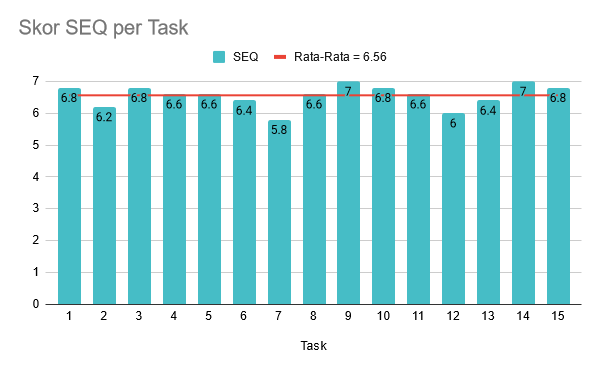
\includegraphics[width=0.6\textwidth]{hifi2/hasil-seq.png}
    \caption{Hasil \textit{Single Ease Question} Pengujian Prototipe \textit{High-Fidelity} Iterasi Pertama dan Kedua}
    \label{img:seq_2}
  \end{figure}
  \FloatBarrier

  \item \textit{System Usability Scale} (SUS)
  \subitem  Berdasarkan hasil nilai SUS pada Gambar \ref{img:sus_2}, terlihat bahwa nilai yang diberikan setiap partisipan untuk \textit{usability} dari prototipe mengalami peningkatan, terutama dari partisipan 3. Hal tersebut membuat nilai rata-rata SUS meningkat dari 82,5 menjadi 91,5. Menurut studi pada Bab \ref{subsubsec:sus}, nilai tersebut tersebut termasuk ke dalam kategori A. Dari penilaian tersebut, dapat disebutkan bahwa prototipe \textit{high-fidelity} iterasi kedua memiliki tingkat \textit{usability} lebih baik daripada prototipe iterasi pertama.

  \begin{figure}[h]
    \centering
    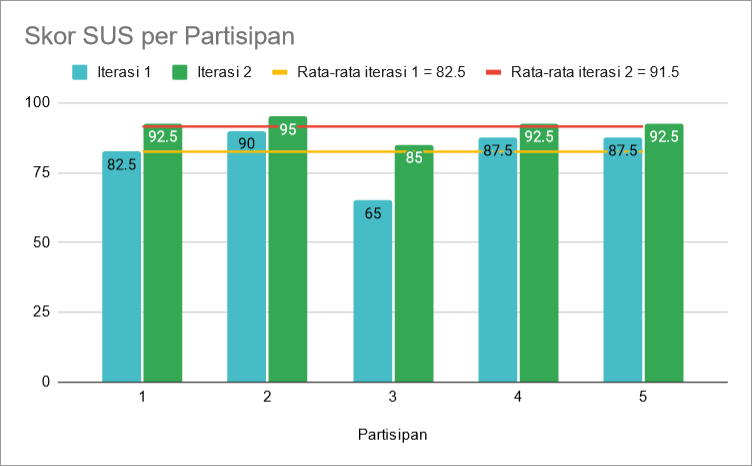
\includegraphics[width=0.6\textwidth]{hifi2/hasil-sus.png}
    \caption{Hasil \textit{System Usability Scale} Pengujian Prototipe \textit{High-Fidelity} Iterasi Pertama dan Kedua}
    \label{img:sus_2}
  \end{figure}
  \FloatBarrier

  \item \textit{Intrinsic Motivation Inventory} (IMI)
  \subitem  Berdasarkan Gambar \ref{img:imi1_2} dapat dilihat bahwa skor IMI untuk subskala \textit{Value/Usefulness} yang dicapai prototipe \textit{high-fidelity} iterasi kedua memiliki rata-rata 6,89, meningkat dari prototipe iterasi pertama sebesar 6,46. Dengan demikian, partisipan setuju rancangan prototipe \textit{high-fidelity} iterasi kedua lebih baik dalam mengarah ke \textit{user experience goal helpful} daripada iterasi sebelumnya.
  
  \begin{figure}[h]
    \centering
    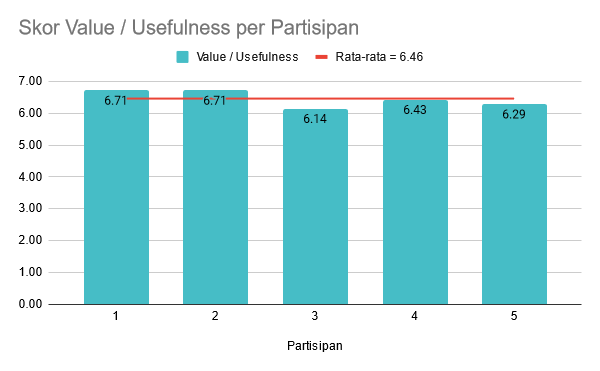
\includegraphics[width=0.6\textwidth]{hifi2/hasil-imi1.png}
    \caption{Hasil \textit{Intrinsic Motivation Inventory} Subskala \textit{Value/Usefulness} Pengujian Prototipe \textit{High-Fidelity} Iterasi Pertama dan Kedua}
    \label{img:imi1_2}
  \end{figure}
  \FloatBarrier
  
  \subitem  Berdasarkan Gambar \ref{img:imi2_2} dapat dilihat bahwa skor IMI untuk subskala \textit{Interest/Enjoyment} mengalami peningkatan pada prototipe \textit{high-fidelity} iterasi kedua, dari rata-rata skor 5,69 menjadi 6,2. Hal ini menunjukkan bahwa perbaikan pada prototipe yang meningkatkan \textit{usability}, dapat meningkatkan juga tingkat motivasi pengguna dari menggunakan prototipe. Adapun skor IMI untuk subskala \textit{Pressure/Tension} yang mengalami penurunan dari rata-rata skor 1,48 menjadi 1,36. Penurunan ini dapat dilihat sebagai peningkatan kualitas desain, dengan maksud prototipe \textit{high-fidelity} iterasi kedua lebih tidak membuat penggunanya merasa tertekan. Kedua hal tersebut menunjukkan bahwa prototipe iterasi kedua dapat mengarah ke \textit{user experience goal motivating} dengan lebih baik.

  \begin{figure}[h]
    \centering
    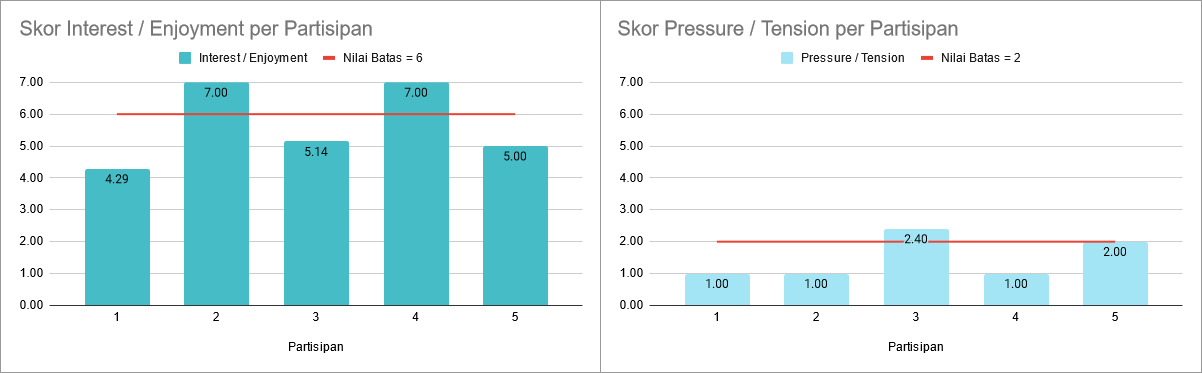
\includegraphics[width=\textwidth]{hifi2/hasil-imi2.png}
    \caption{Hasil \textit{Intrinsic Motivation Inventory} Subskala \textit{Interest/Enjoyment} dan \textit{Pressure/Tension} Pengujian Prototipe \textit{High-Fidelity} Iterasi Pertama dan Kedua}
    \label{img:imi2_2}
  \end{figure}
  \FloatBarrier

\end{enumerate}